\begin{enumerate}[label={},font=\normalfont,leftmargin=1.15cm,labelwidth=1.0cm,labelsep=0.15cm,itemindent=0pt,listparindent=0pt,parsep=0pt,topsep=0pt]
\item[4.1.4] If $PQ$ and $PR$ are tangents to the circle with centre $O$ and radius $4$ cm such that $\angle QPR=90^\circ$, find the length $OP$.

\begin{multicols}{4}
\begin{enumerate}
\setlength{\itemsep}{0pt}
    \item $4$ cm
    \item $4\sqrt{2}$ cm
    \item $8$ cm
    \item $2\sqrt{2}$ cm
\end{enumerate}
\end{multicols}

\vspace{0.7em}\par\solution


The radii to the points of contact are perpendicular to the tangents, so $\angle OQP=90^\circ$ and $\angle ORP=90^\circ$. The right triangles $\triangle OPQ$ and $\triangle OPR$ are congruent, so $OP$ bisects $\angle QPR$. Hence $\angle QPO=45^\circ$. In right triangle $OPQ$,
\begin{equation*}
\sin 45^\circ=\frac{OQ}{OP}=\frac{4}{OP},
\qquad OP=4\sqrt{2}\text{ cm}.
\tag*{(\ref{formula-1-1-1})}\end{equation*}
Therefore, the correct answer is \textbf{b)}.

The following code draws the tangent configuration and calculates $OP$.
\begin{lstlisting}[frame=single, basicstyle=\rmfamily, escapeinside={(*@}{@*)}]
(*@\makebox[\dimexpr\linewidth-2\fboxsep-2\fboxrule\relax][c]{codes/4.1.4.py}@*)
\end{lstlisting}
\begin{figure}[H]
    \centering
    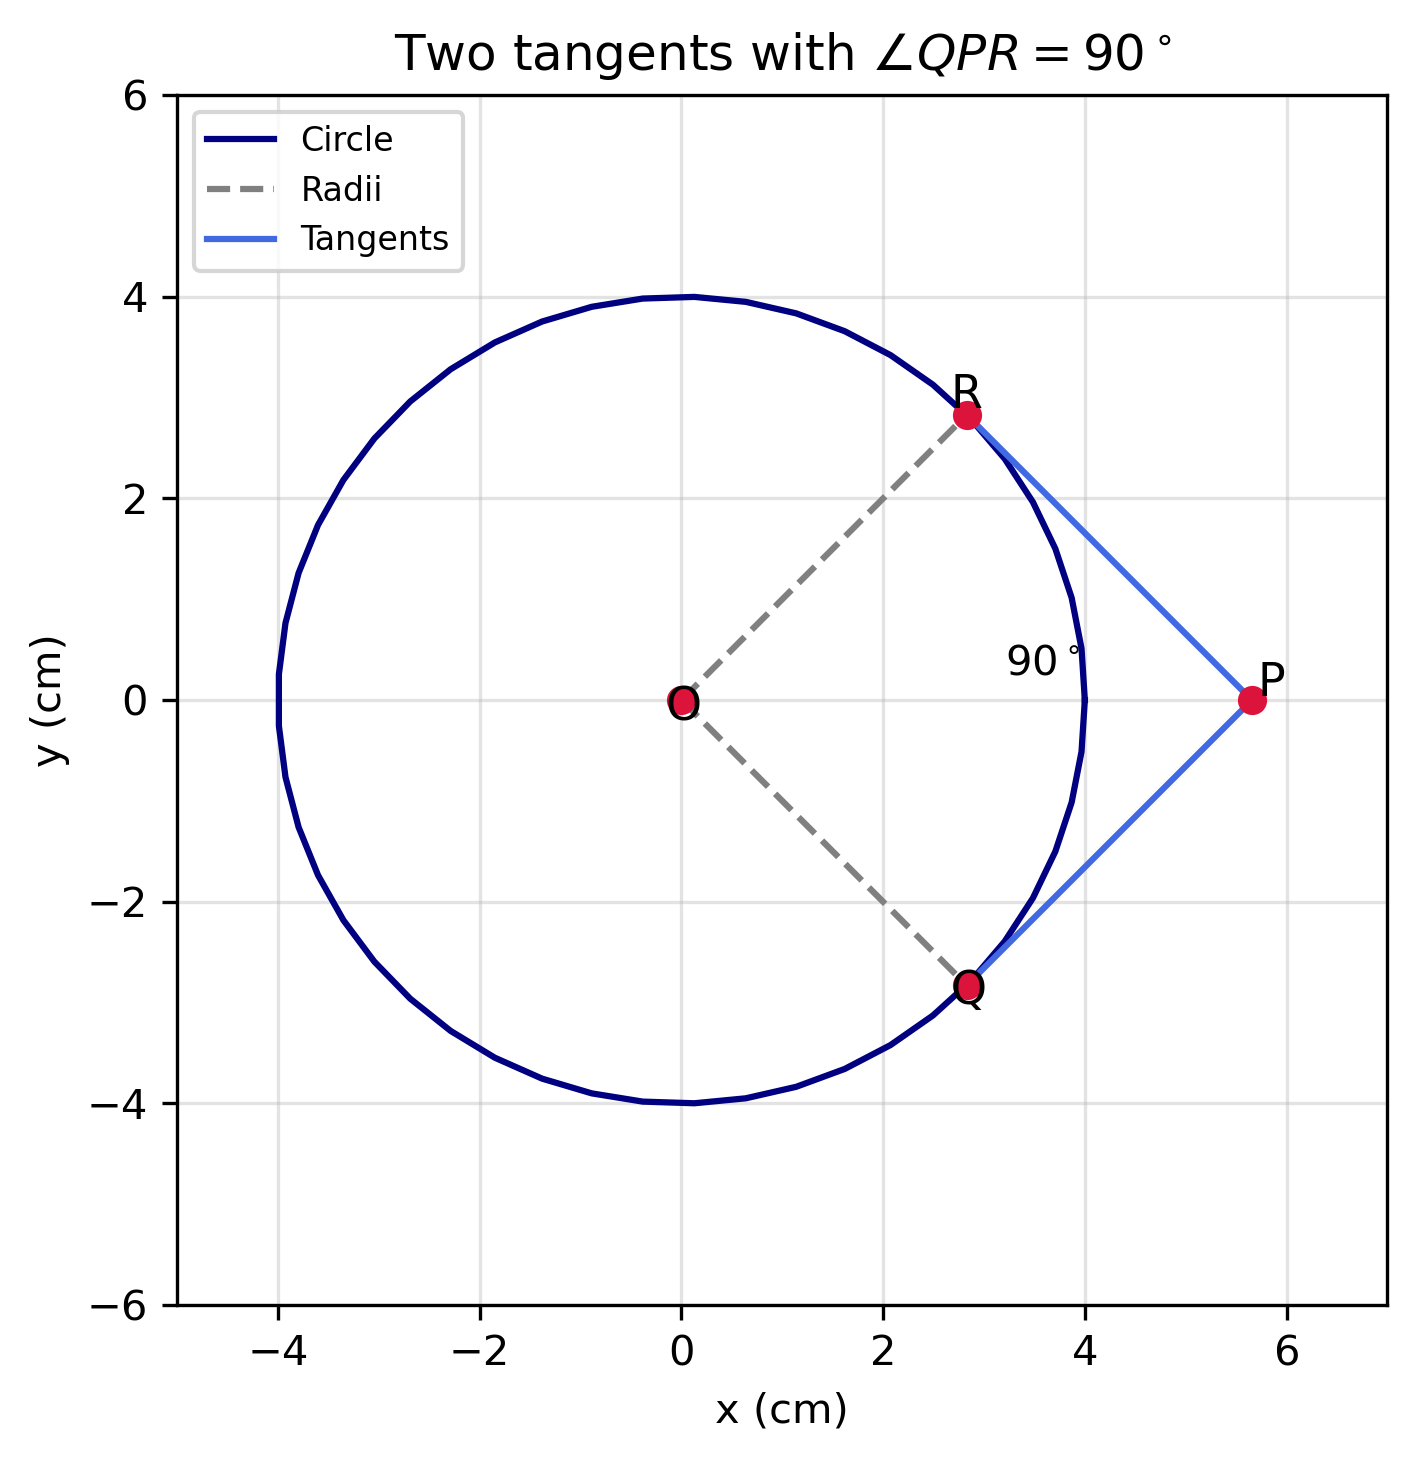
\includegraphics[width=0.62\linewidth]{figs/4.1.4.png}
    \caption{Tangents $PQ$ and $PR$ to a circle of radius $4$ cm, with $\angle QPR=90^\circ$.}
    \label{fig:4.1.4}
\end{figure}
\end{enumerate}

\newpage
\begin{enumerate}[label={},font=\normalfont,leftmargin=1.15cm,labelwidth=1.0cm,labelsep=0.15cm,itemindent=0pt,listparindent=0pt,parsep=0pt,topsep=0pt]
\item[4.1.7] In the given figure, a circle is centred at $(1,2)$. Find the diameter of the circle.

\begin{multicols}{4}
\begin{enumerate}
\setlength{\itemsep}{0pt}
    \item $4$
    \item $2\sqrt{2}$
    \item $\sqrt{5}$
    \item $2\sqrt{5}$
\end{enumerate}
\end{multicols}

\vspace{0.7em}\par\solution


From the figure, the endpoints of the diameter are $(0,4)$ and $(2,0)$. Their midpoint is $(1,2)$, the given centre. Hence the diameter is
\begin{equation*}
\sqrt{(2-0)^2+(0-4)^2}=\sqrt{4+16}=2\sqrt{5}.
\tag*{(\ref{formula-1-1-2})}\end{equation*}
The correct answer is \textbf{d)}.

The following code plots the circle and diameter, then calculates the diameter.
\begin{lstlisting}[frame=single, basicstyle=\rmfamily, escapeinside={(*@}{@*)}]
(*@\makebox[\dimexpr\linewidth-2\fboxsep-2\fboxrule\relax][c]{codes/4.1.7.py}@*)
\end{lstlisting}
\begin{figure}[H]
    \centering
    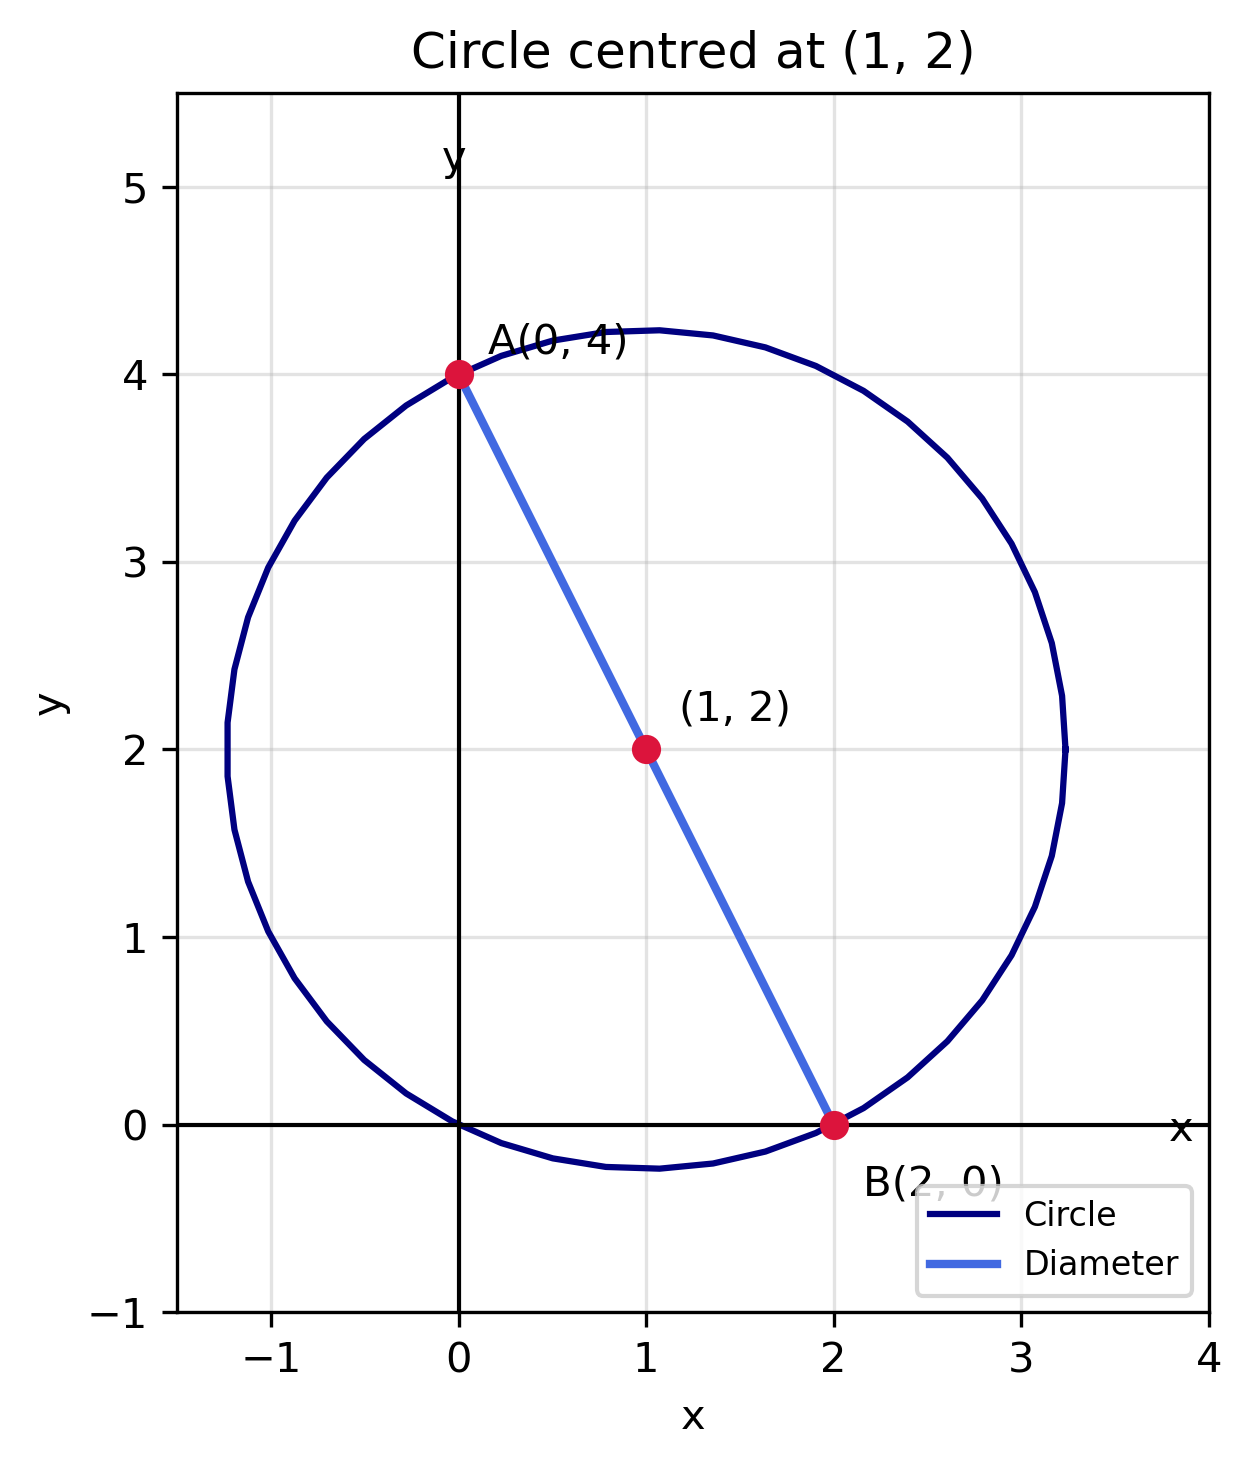
\includegraphics[width=0.56\linewidth]{figs/4.1.7.png}
    \caption{Circle centred at $(1,2)$ with the diameter endpoints shown.}
    \label{fig:4.1.7}
\end{figure}
\end{enumerate}


\newpage
\begin{enumerate}[label={},font=\normalfont,leftmargin=1.15cm,labelwidth=1.0cm,labelsep=0.15cm,itemindent=0pt,listparindent=0pt,parsep=0pt,topsep=0pt]
\item[4.1.8] The value of $k$ for which the system of linear equations $\dfrac{x}{2}+\dfrac{y}{3}=5$ and $2x+ky=7$ is inconsistent, is:

\begin{multicols}{4}
\begin{enumerate}
\setlength{\itemsep}{0pt}
    \item $\dfrac{3}{4}$
    \item $\dfrac{4}{3}$
    \item $\dfrac{1}{3}$
    \item $3$
\end{enumerate}
\end{multicols}

\vspace{0.7em}\par\solution


The first equation is $3x+2y=30$. For the two lines to be parallel, $\dfrac{3}{2}=\dfrac{2}{k}$, so $k=\dfrac{4}{3}$. Their constant terms are not in the same ratio, so the lines are distinct and the system is inconsistent. The correct answer is \textbf{b)}.\par\noindent\hfill\mbox{\textit{(\ref{formula-1-1-3})}}\par

The following code plots the two parallel lines.
\begin{lstlisting}[frame=single, basicstyle=\rmfamily, escapeinside={(*@}{@*)}]
(*@\makebox[\dimexpr\linewidth-2\fboxsep-2\fboxrule\relax][c]{codes/4.1.8.py}@*)
\end{lstlisting}
\begin{figure}[H]
    \centering
    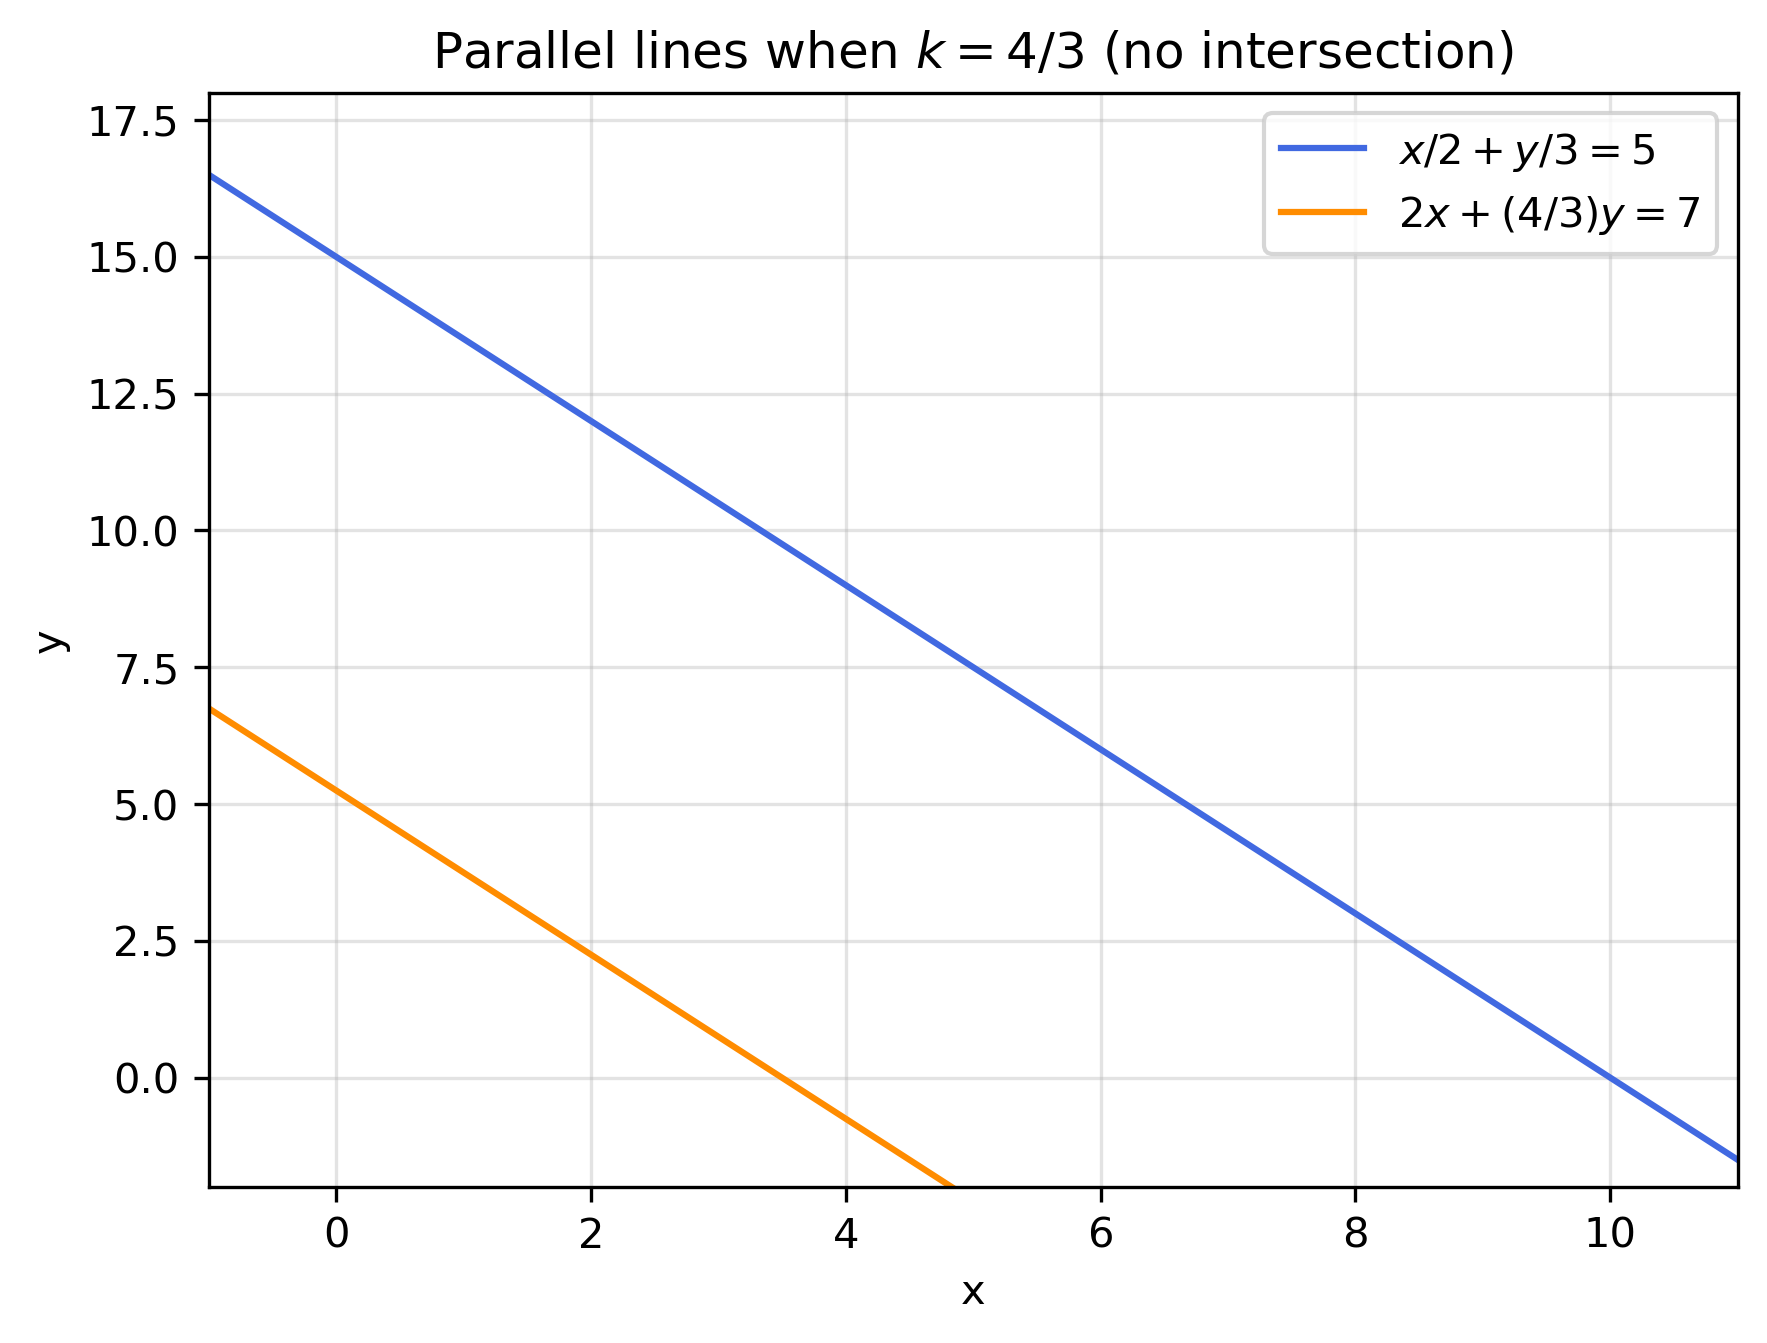
\includegraphics[width=0.58\linewidth]{figs/4.1.8.png}
    \caption{The parallel lines for $k=\dfrac{4}{3}$; they have no point of intersection.}
    \label{fig:4.1.8}
\end{figure}
\end{enumerate}

\vspace{1.2em}
\newpage
\begin{enumerate}[label={},font=\normalfont,leftmargin=1.15cm,labelwidth=1.0cm,labelsep=0.15cm,itemindent=0pt,listparindent=0pt,parsep=0pt,topsep=0pt]
\item[4.1.10] Two different dice are rolled together. Find the probability that both obtained numbers are less than $4$.

\begin{multicols}{4}
\begin{enumerate}
\setlength{\itemsep}{0pt}
    \item $\dfrac{2}{9}$
    \item $\dfrac{7}{36}$
    \item $\dfrac{1}{4}$
    \item $\dfrac{2}{3}$
\end{enumerate}
\end{multicols}

\vspace{0.7em}\par\solution


Each die can show $1$, $2$, or $3$, giving $3\times3=9$ favourable outcomes out of $36$ equally likely outcomes. Thus, $P=\dfrac{9}{36}=\dfrac{1}{4}$. The correct answer is \textbf{c)}. The code simulates $500{,}000$ rolls and plots the empirical and theoretical probability distributions for the event.\par\noindent\hfill\mbox{\textit{(\ref{formula-1-1-4})}}\par

\begin{lstlisting}[frame=single, basicstyle=\rmfamily, escapeinside={(*@}{@*)}]
(*@\makebox[\dimexpr\linewidth-2\fboxsep-2\fboxrule\relax][c]{codes/4.1.10.py}@*)
\end{lstlisting}
\begin{figure}[H]
    \centering
    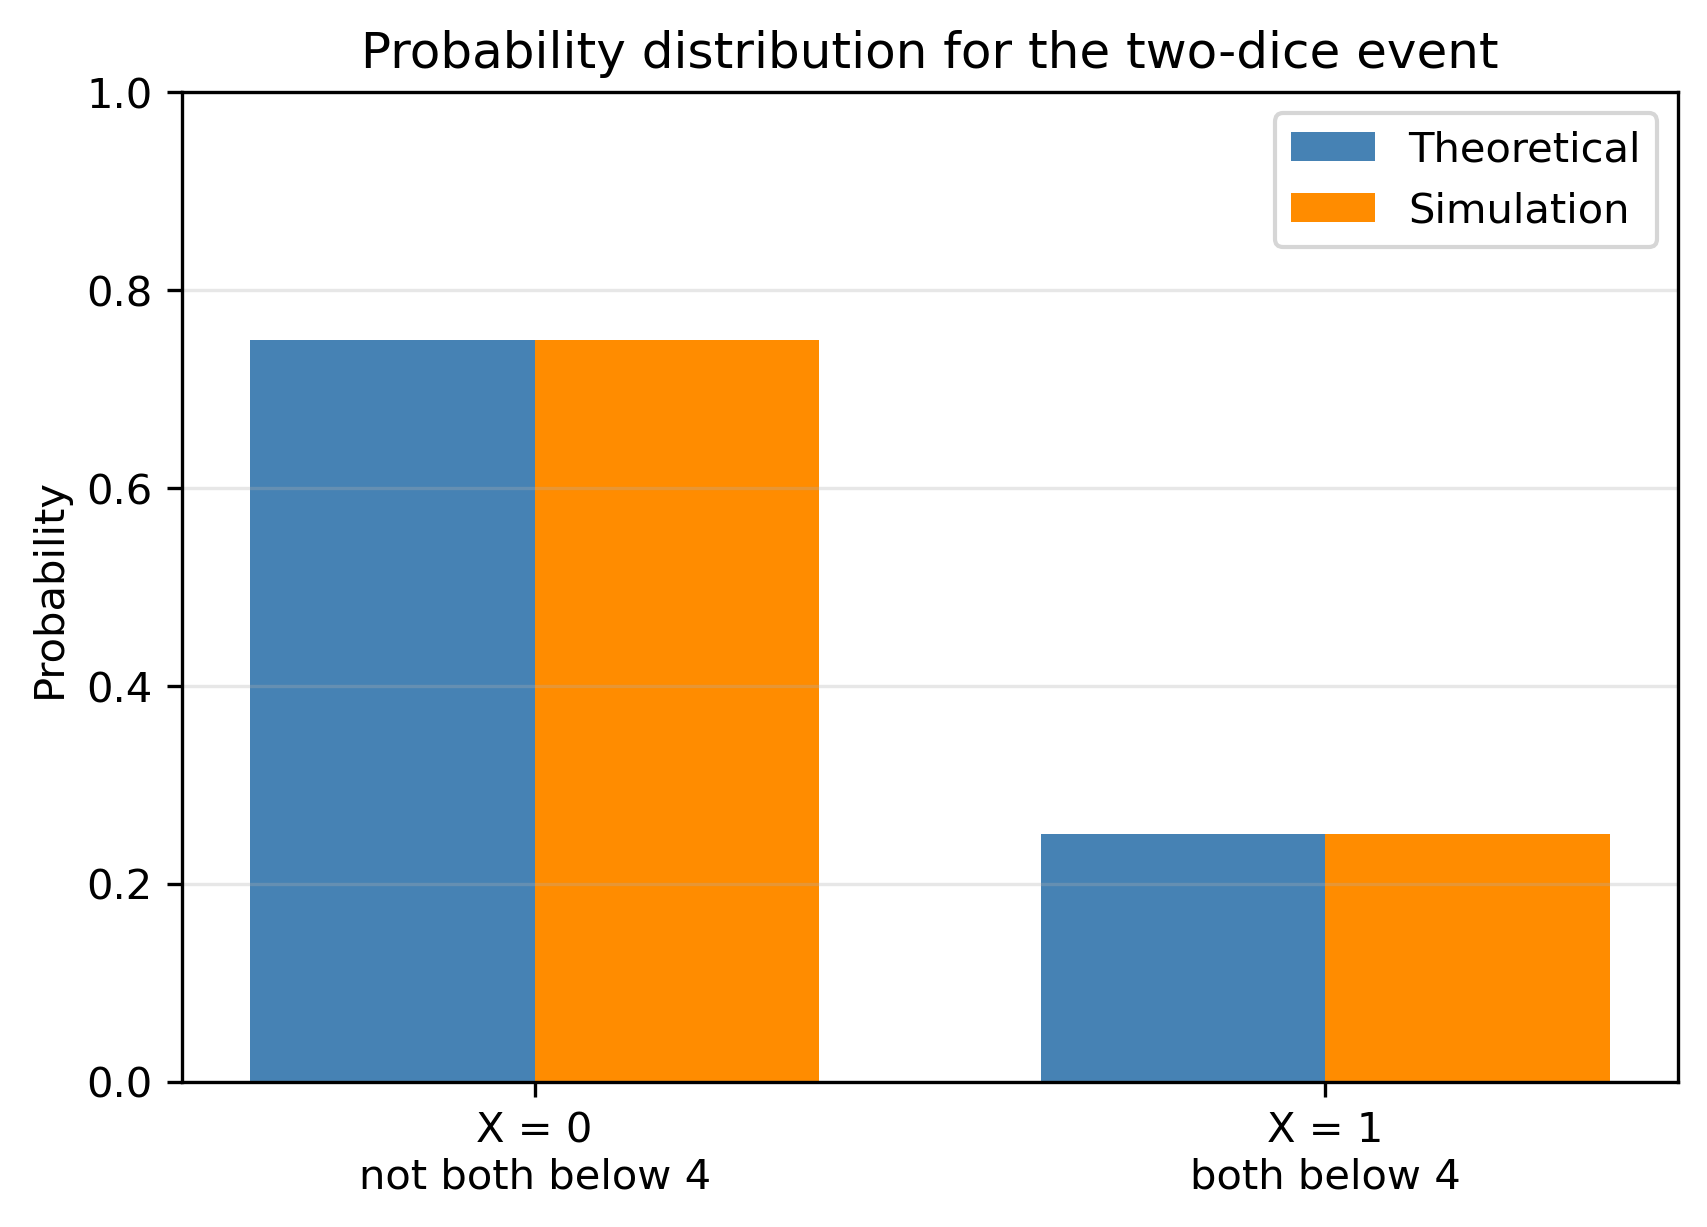
\includegraphics[width=0.56\linewidth]{figs/4.1.10.png}
    \caption{Probability distribution of $X$, where $X=1$ if both dice show a number below $4$, and $X=0$ otherwise.}
    \label{fig:4.1.10}
\end{figure}
\end{enumerate}

\vspace{1.2em}
\newpage
\begin{enumerate}[label={},font=\normalfont,leftmargin=1.15cm,labelwidth=1.0cm,labelsep=0.15cm,itemindent=0pt,listparindent=0pt,parsep=0pt,topsep=0pt]
\item[4.1.14] $PQ$ is tangent to a circle with centre $O$. If $\angle POR=65^\circ$, find $m\angle PTR$.

\begin{multicols}{4}
\begin{enumerate}
\setlength{\itemsep}{0pt}
    \item $65^\circ$
    \item $58.5^\circ$
    \item $57.5^\circ$
    \item $45^\circ$
\end{enumerate}
\end{multicols}

\vspace{0.7em}\par\solution


Since $OP$ is a radius to the point of tangency, $OP\perp PQ$, so $\angle SPT=90^\circ$. The inscribed angle $\angle PSR$ subtending arc $PR$ is half the central angle $\angle POR$, hence $\angle PST=\angle PSR=32.5^\circ$ because $S$, $R$, and $T$ are collinear. Therefore, in $\triangle PST$,
\begin{equation*}
\angle PTR=\angle PTS=180^\circ-90^\circ-32.5^\circ=57.5^\circ.
\tag*{(\ref{formula-1-1-1})}\end{equation*}
The correct answer is \textbf{c)}.

The following code draws the circle, tangent and secant, and calculates $\angle PTR$.
\begin{lstlisting}[frame=single, basicstyle=\rmfamily, escapeinside={(*@}{@*)}]
(*@\makebox[\dimexpr\linewidth-2\fboxsep-2\fboxrule\relax][c]{codes/4.1.14.py}@*)
\end{lstlisting}
\begin{figure}[H]
    \centering
    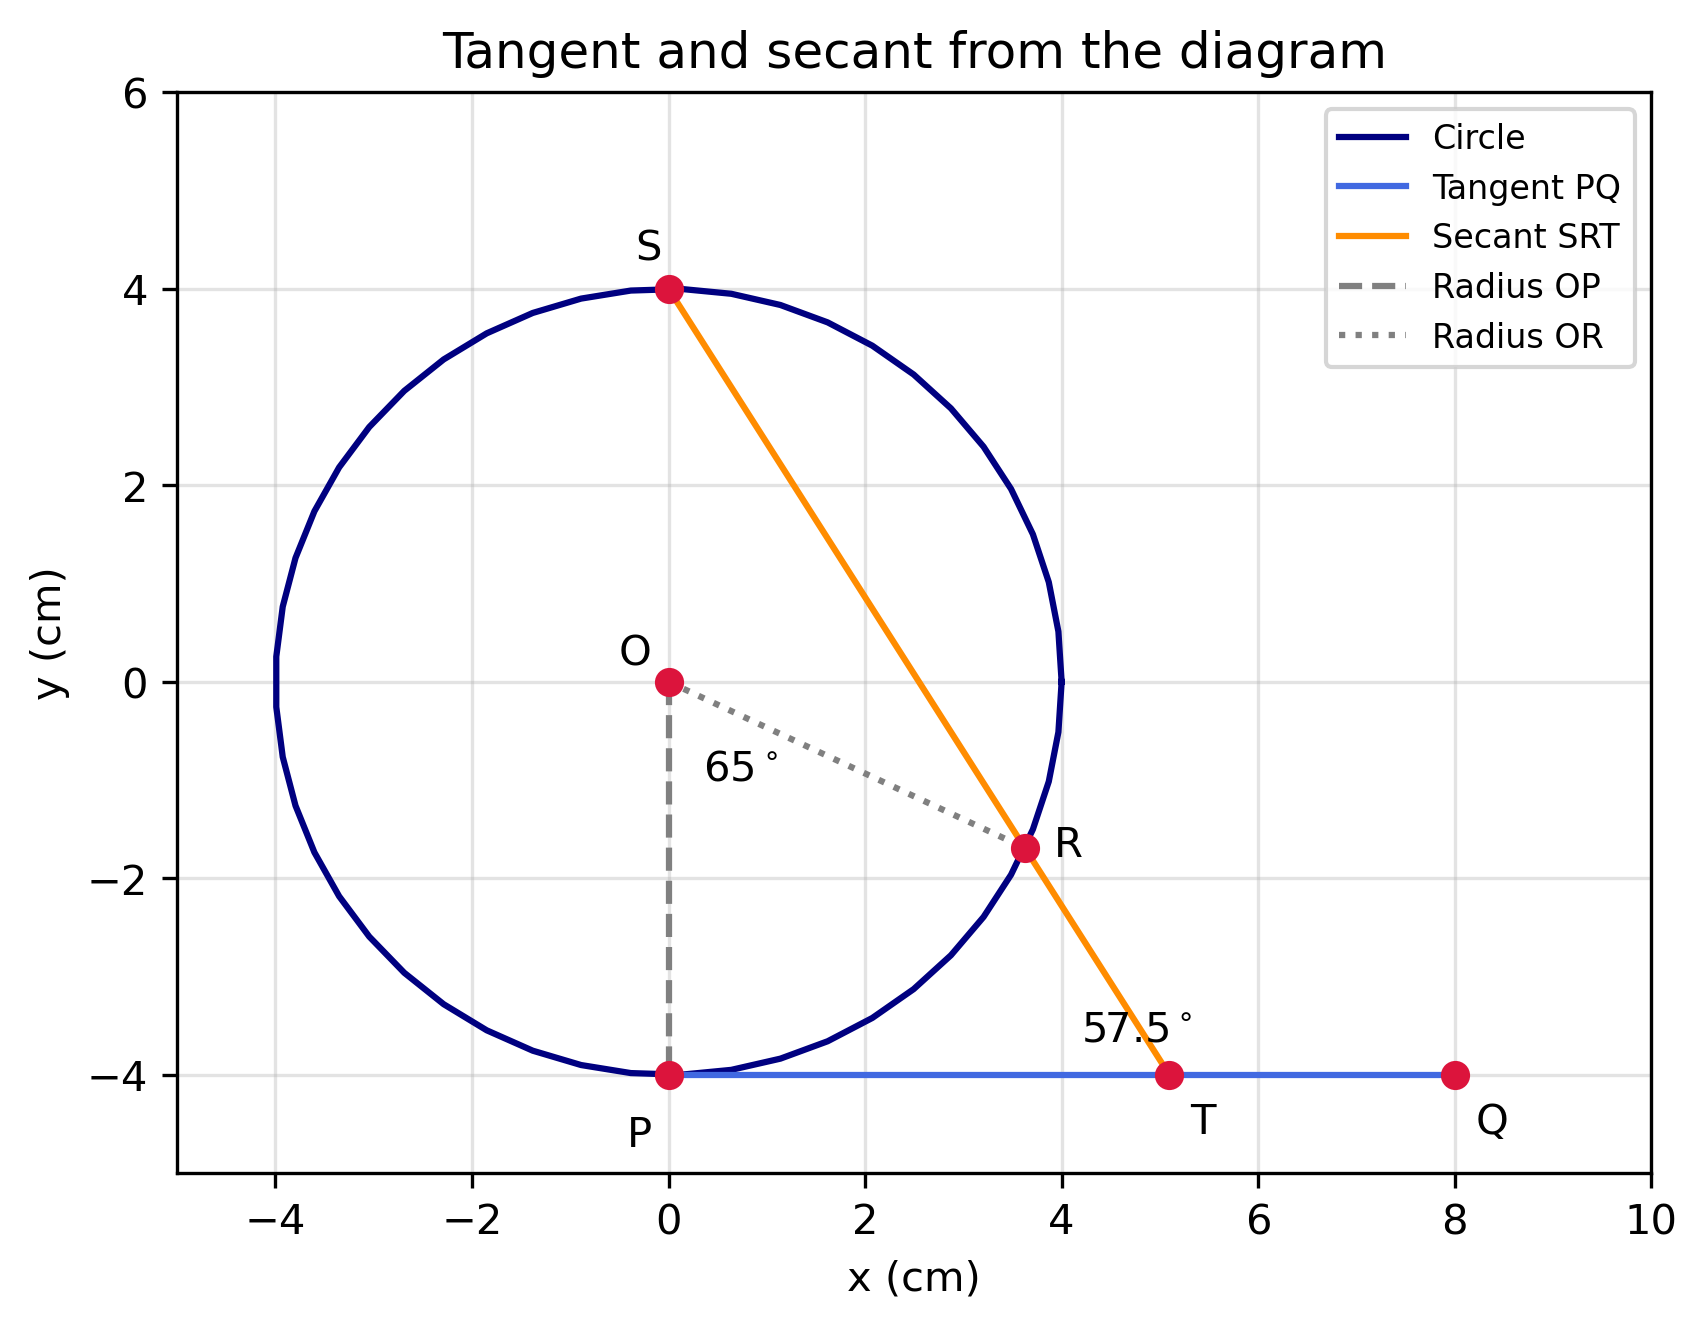
\includegraphics[width=0.58\linewidth]{figs/4.1.14.png}
    \caption{Tangent $PQ$ and secant $SRT$ with central angle $\angle POR=65^\circ$.}
    \label{fig:4.1.14}
\end{figure}
\end{enumerate}

\newpage
\begin{enumerate}[label={},font=\normalfont,leftmargin=1.15cm,labelwidth=1.0cm,labelsep=0.15cm,itemindent=0pt,listparindent=0pt,parsep=0pt,topsep=0pt]
\item[4.1.17] Arc $PQ$ subtends an angle $\theta$ at the centre of a circle of radius $6.3$ cm. If the length of arc $PQ$ is $11$ cm, find $\theta$.

\begin{multicols}{4}
\begin{enumerate}
\setlength{\itemsep}{0pt}
    \item $10^\circ$
    \item $60^\circ$
    \item $45^\circ$
    \item $100^\circ$
\end{enumerate}
\end{multicols}

\vspace{0.7em}\par\solution


Using arc length $s=r\theta$ (with $\theta$ in radians),
\begin{equation*}
\theta=\frac{11}{6.3}\text{ radians}=100^\circ.
\tag*{(\ref{formula-1-1-7})}\end{equation*}
The correct answer is \textbf{d)}.

The code draws the arc and radii, and calculates the angle.
\begin{lstlisting}[frame=single, basicstyle=\rmfamily, escapeinside={(*@}{@*)}]
(*@\makebox[\dimexpr\linewidth-2\fboxsep-2\fboxrule\relax][c]{codes/4.1.17.py}@*)
\end{lstlisting}
\begin{figure}[H]
    \centering
    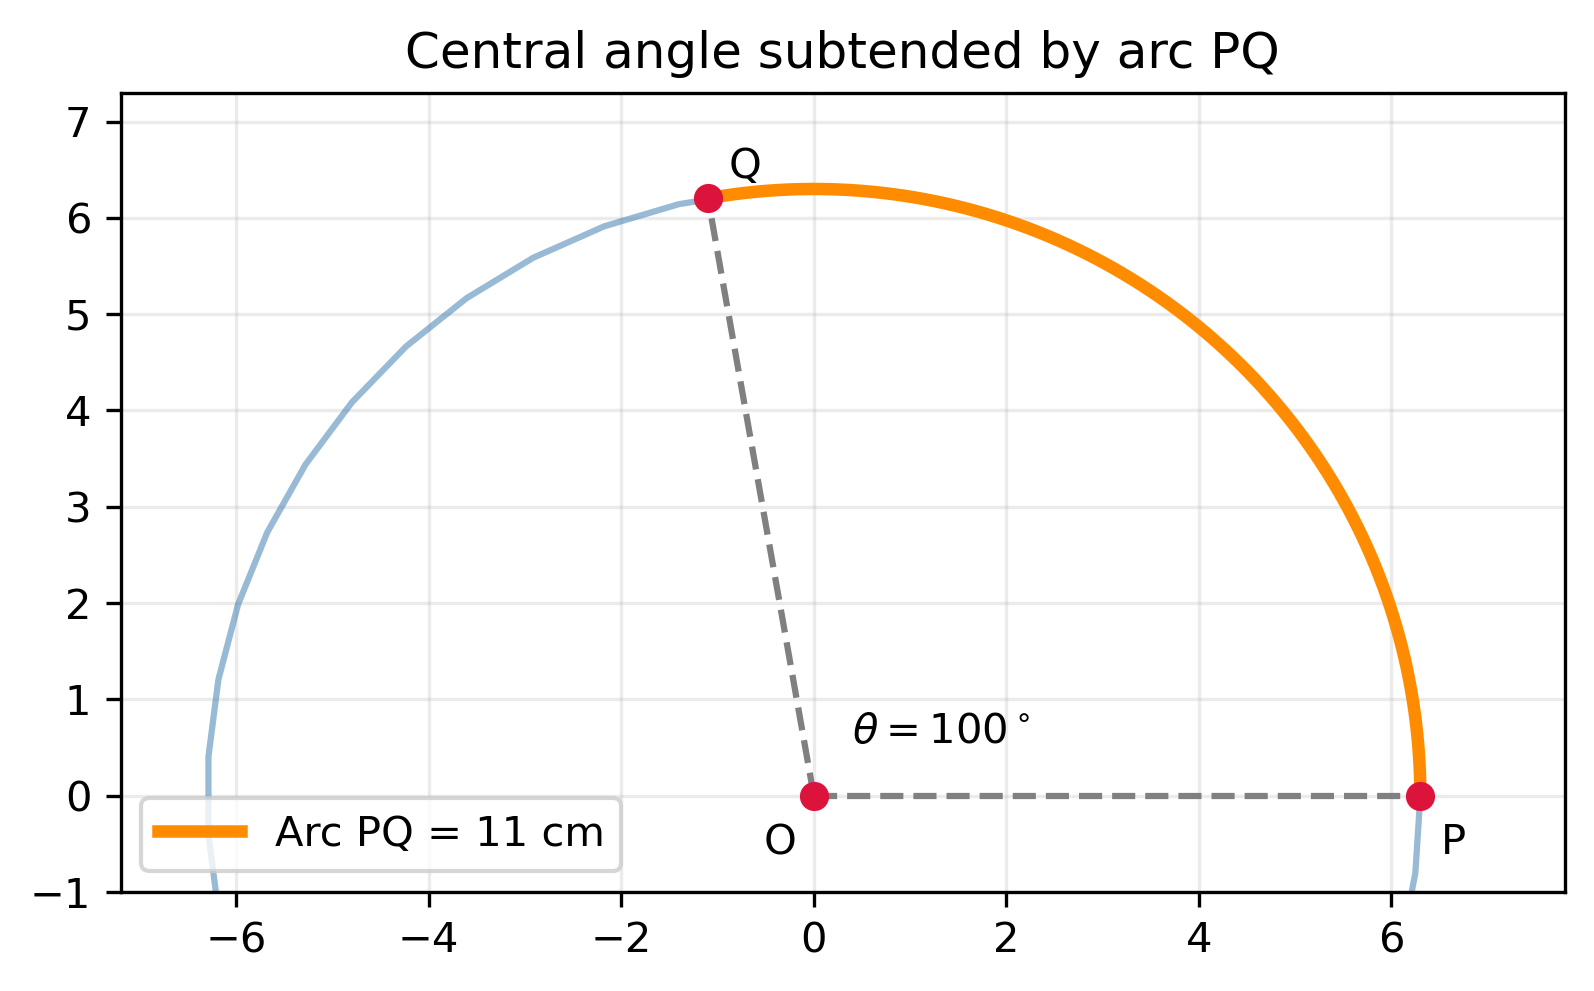
\includegraphics[width=0.53\linewidth]{figs/4.1.17.png}
    \caption{Arc $PQ$ of length $11$ cm subtending $100^\circ$ at the centre.}
\end{figure}
\end{enumerate}

\vspace{1.2em}
\begin{enumerate}[label={},font=\normalfont,leftmargin=1.15cm,labelwidth=1.0cm,labelsep=0.15cm,itemindent=0pt,listparindent=0pt,parsep=0pt,topsep=0pt]
\item[4.1.21] Verify that the roots of $(p-q)x^2+(q-r)x+(r-p)=0$ are equal when $q+r=2p$.

\vspace{0.7em}\par\solution


Put $r=2p-q$. Then the equation becomes
\begin{equation*}
(p-q)x^2+2(q-p)x+(p-q)=0
\quad\Longrightarrow\quad
(p-q)(x-1)^2=0.
\tag*{(\ref{formula-1-1-5})}\end{equation*}
Thus both roots are $x=1$ (for the non-degenerate quadratic case), so the roots are equal.
\end{enumerate}

\vspace{1.2em}
\begin{enumerate}[label={},font=\normalfont,leftmargin=1.15cm,labelwidth=1.0cm,labelsep=0.15cm,itemindent=0pt,listparindent=0pt,parsep=0pt,topsep=0pt]
\item[4.1.22] $D$ is a point on side $BC$ of $\triangle ABC$ such that $\angle CAB=\angle CDA$. Show that $CA^2=CB\times CD$.

\vspace{0.7em}\par\solution


Since $D$ lies on $BC$, $\angle ACB=\angle DCA$. With the given $\angle CAB=\angle CDA$, $\triangle CAB\sim\triangle CDA$ (AA). Corresponding sides give
\begin{equation*}
\frac{CA}{CD}=\frac{CB}{CA},
\qquad\therefore\qquad CA^2=CB\times CD.
\tag*{(\ref{formula-1-1-6})}\end{equation*}

The following code draws a configuration satisfying the given angles and verifies the proportionality numerically.
\begin{lstlisting}[frame=single, basicstyle=\rmfamily, escapeinside={(*@}{@*)}]
(*@\makebox[\dimexpr\linewidth-2\fboxsep-2\fboxrule\relax][c]{codes/4.1.22.py}@*)
\end{lstlisting}
\begin{figure}[H]
    \centering
    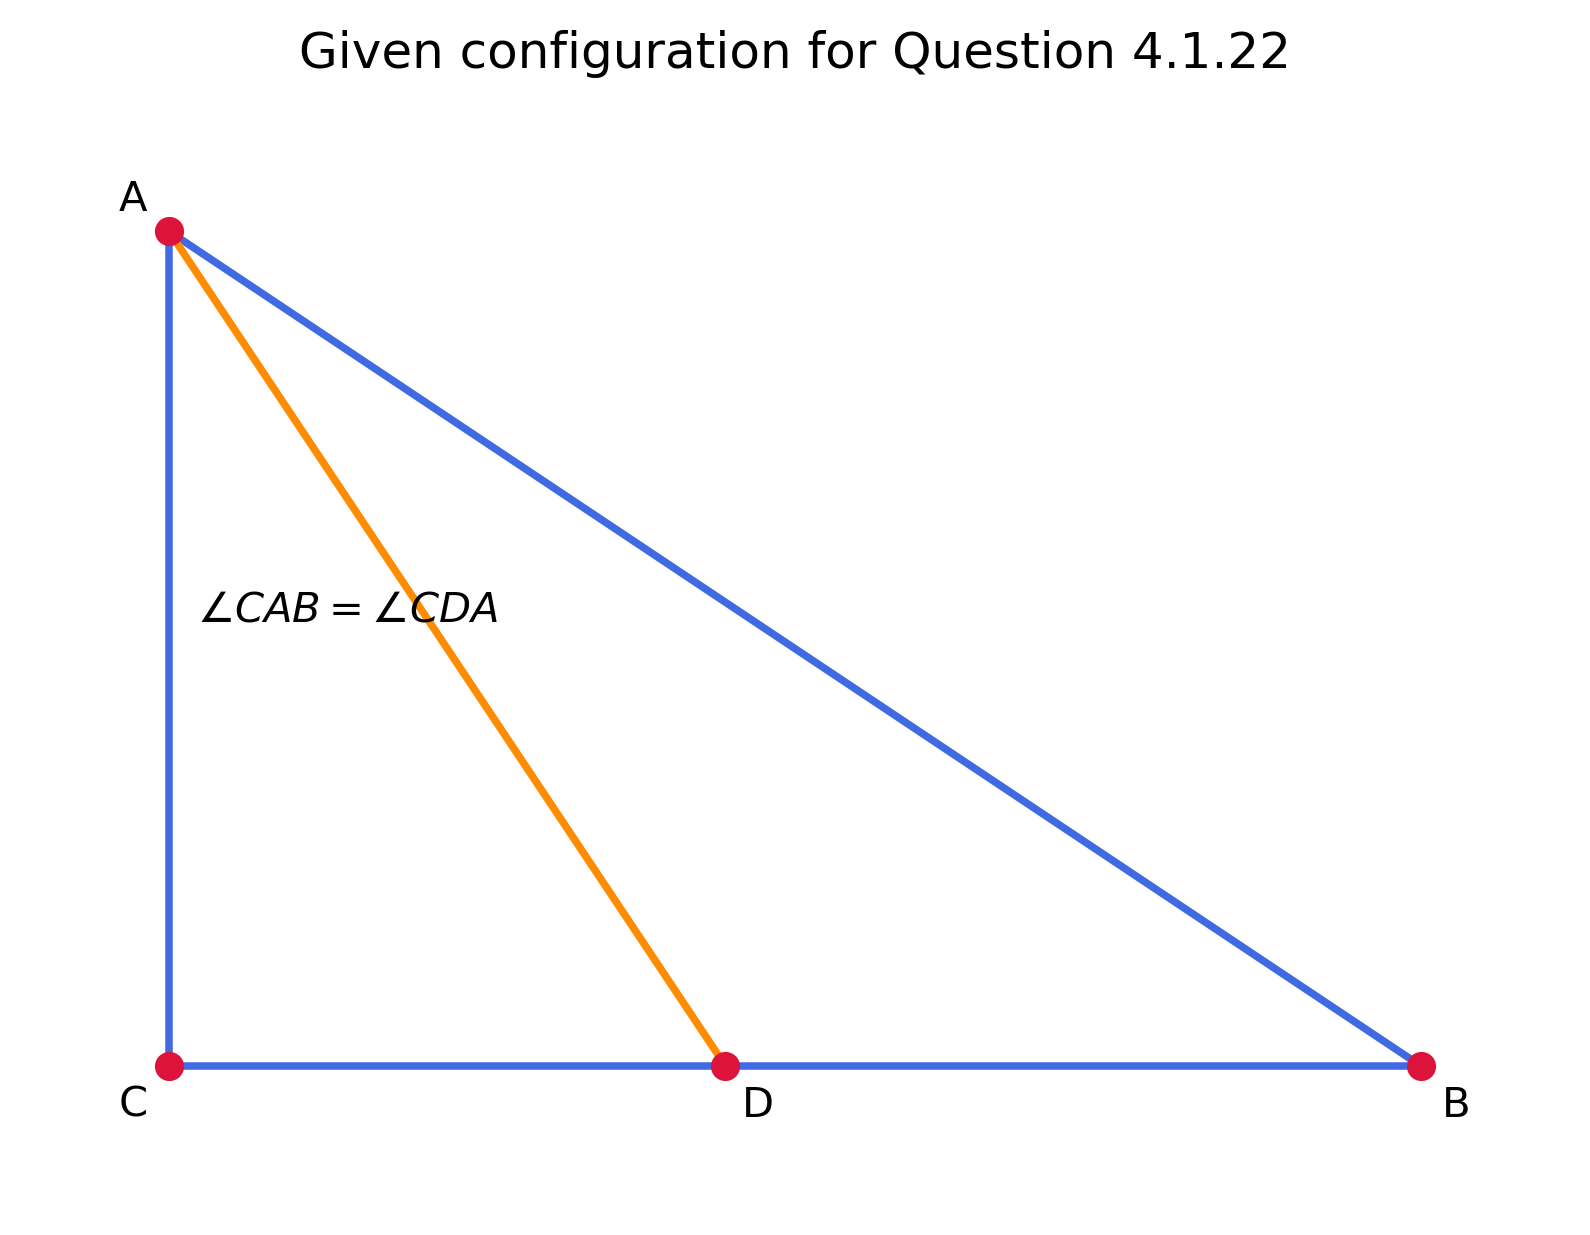
\includegraphics[width=0.50\linewidth]{figs/4.1.22.png}
    \caption{Triangle $ABC$ with $D$ on $BC$ and $AD$ drawn.}
\end{figure}
\end{enumerate}

\vspace{1.2em}
\begin{enumerate}[label={},font=\normalfont,leftmargin=1.15cm,labelwidth=1.0cm,labelsep=0.15cm,itemindent=0pt,listparindent=0pt,parsep=0pt,topsep=0pt]
\item[4.1.26.1] In a class test, Veer scored 6 more than twice Kevin's marks. If one of them had scored 4 more marks, their total would have been 40. Find Veer's and Kevin's marks.

\vspace{0.7em}\par\solution

Let Kevin's marks be $K$ and Veer's be $V$. Then $V=2K+6$ and $V+K+4=40$, so $3K+10=40$. Thus $K=10$ and $V=26$ marks.

The code plots the two relationships and marks their intersection.
\begin{lstlisting}[frame=single, basicstyle=\rmfamily, escapeinside={(*@}{@*)}]
(*@\makebox[\dimexpr\linewidth-2\fboxsep-2\fboxrule\relax][c]{codes/4.1.26.1.py}@*)
\end{lstlisting}
\begin{figure}[H]
    \centering
    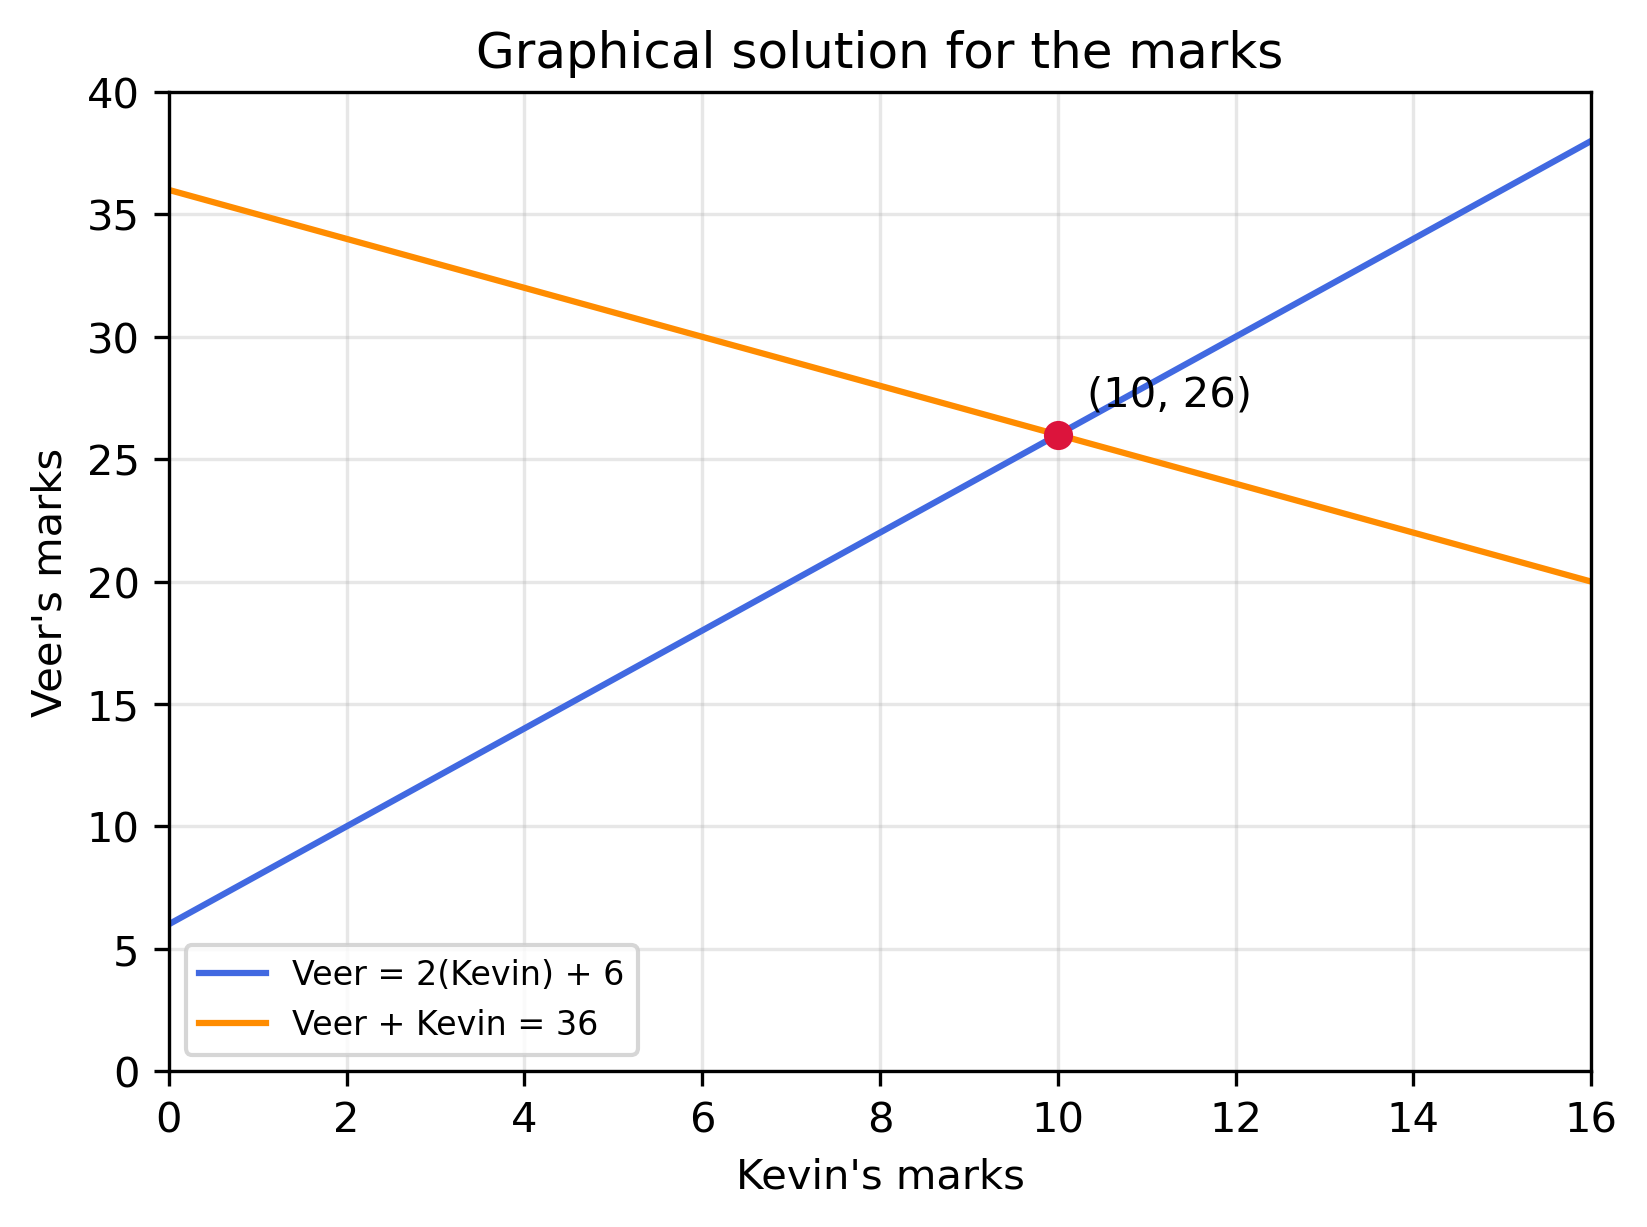
\includegraphics[width=0.50\linewidth]{figs/4.1.26.1.png}
    \caption{Veer and Kevin's marks at the intersection of the two lines.}
\end{figure}

\item[4.1.26.2] Solve the linear equations $3x+y=14$ and $y=2$ graphically.

\vspace{0.7em}\par\solution


The lines $y=14-3x$ and $y=2$ intersect at $(4,2)$. Hence the solution is $\boxed{x=4,\ y=2}$.\par\noindent\hfill\mbox{\textit{(\ref{formula-1-1-3})}}\par

The code plots both lines and marks their intersection.
\begin{lstlisting}[frame=single, basicstyle=\rmfamily, escapeinside={(*@}{@*)}]
(*@\makebox[\dimexpr\linewidth-2\fboxsep-2\fboxrule\relax][c]{codes/4.1.26.2.py}@*)
\end{lstlisting}
\begin{figure}[H]
    \centering
    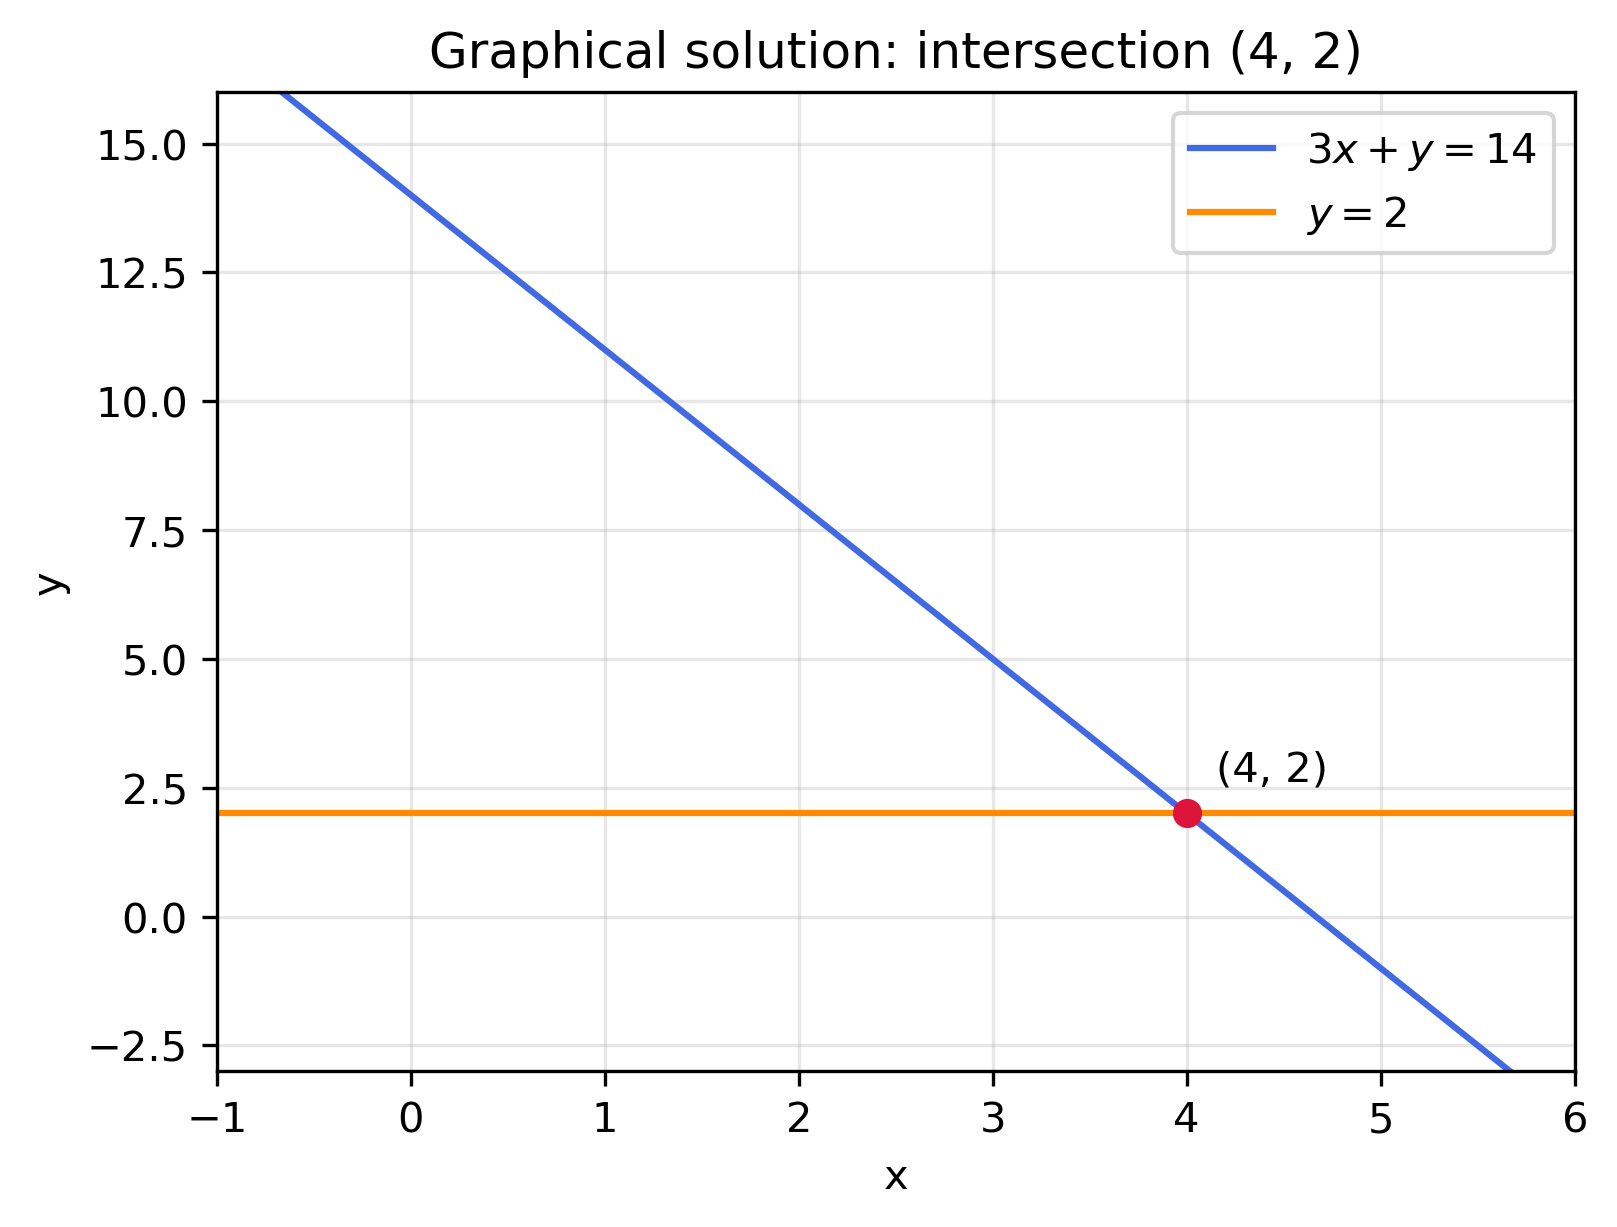
\includegraphics[width=0.52\linewidth]{figs/4.1.26.2.png}
    \caption{Graphical solution of the pair of linear equations.}
\end{figure}
\end{enumerate}

\newpage
\begin{enumerate}[label={},font=\normalfont,leftmargin=1.15cm,labelwidth=1.0cm,labelsep=0.15cm,itemindent=0pt,listparindent=0pt,parsep=0pt,topsep=0pt]
\item[4.1.30] A bag contains 30 balls, of which $m$ are blue. (i) Find the probability that a ball drawn at random is not blue. (ii) If 6 more blue balls are added, the probability of drawing a blue ball becomes $\frac54$ times its original value. Find $m$.

\vspace{0.7em}\par\solution


(i) The number of non-blue balls is $30-m$, so $P(\text{not blue})=\dfrac{30-m}{30}$.\\
(ii) The new probability is $\dfrac{m+6}{36}$. Therefore
\begin{equation*}
\frac{m+6}{36}=\frac54\cdot\frac{m}{30}
\quad\Longrightarrow\quad m=12.
\tag*{(\ref{formula-1-1-4})}\end{equation*}
There are $12$ blue balls initially.
\end{enumerate}

\vspace{1.2em}
\begin{enumerate}[label={},font=\normalfont,leftmargin=1.15cm,labelwidth=1.0cm,labelsep=0.15cm,itemindent=0pt,listparindent=0pt,parsep=0pt,topsep=0pt]
\item[4.1.31] Find the greatest number less than $10{,}000$ that is exactly divisible by $48$, $60$, and $65$.

\vspace{0.7em}\par\solution


\begin{equation*}
\operatorname{LCM}(48,60,65)=2^4\cdot3\cdot5\cdot13=3120.
\tag*{(\ref{formula-1-1-9})}\end{equation*}
The greatest multiple of $3120$ below $10{,}000$ is $3\times3120=\boxed{9360}$.

The following C program calculates the LCM and the required greatest multiple.
\begin{lstlisting}[frame=single, basicstyle=\rmfamily, escapeinside={(*@}{@*)}]
(*@\makebox[\dimexpr\linewidth-2\fboxsep-2\fboxrule\relax][c]{codes/4.1.31.c}@*)
\end{lstlisting}
\end{enumerate}

\vspace{0.3em}
\begin{enumerate}[label={},font=\normalfont,leftmargin=1.15cm,labelwidth=1.0cm,labelsep=0.15cm,itemindent=0pt,listparindent=0pt,parsep=0pt,topsep=0pt]
\item[4.1.33] In the figure, $TP$ and $TQ$ are tangents to the circle with centre $M$, touching the circle with centre $N$ at $A$ and $B$, respectively. Given $MQ=13$ cm, $NB=8$ cm, $BQ=35$ cm and $TP=80$ cm: (i) name quadrilateral $MQBN$; (ii) determine whether $MN\parallel PA$, with justification; (iii) find $TB$; (iv) find $MN$.

\vspace{0.7em}\par\solution


(i) $MQ\parallel NB$ and both are perpendicular to $QB$, so $MQBN$ is a right trapezium.\\
(ii) No: the centres are $13$ cm and $8$ cm from tangent $PA$; hence $MN$ cannot be parallel to $PA$.\\
(iii) $TQ=TP=80$ cm and $TB=TQ-BQ$, so $TB=80-35=45$ cm.\\
(iv) The centres differ by $35$ cm parallel to $QB$ and by $13-8=5$ cm perpendicular to it. Thus $MN=\sqrt{35^2+5^2}=\boxed{25\sqrt2\text{ cm}}$.\par\noindent\hfill\mbox{\textit{(\ref{formula-1-1-1})}}\par

The code draws the two-circle tangent configuration and prints the answers.
\begin{lstlisting}[frame=single, basicstyle=\rmfamily, escapeinside={(*@}{@*)}]
(*@\makebox[\dimexpr\linewidth-2\fboxsep-2\fboxrule\relax][c]{codes/4.1.33.py}@*)
\end{lstlisting}
\vspace{-0.6em}
\begin{figure}[H]
    \centering
    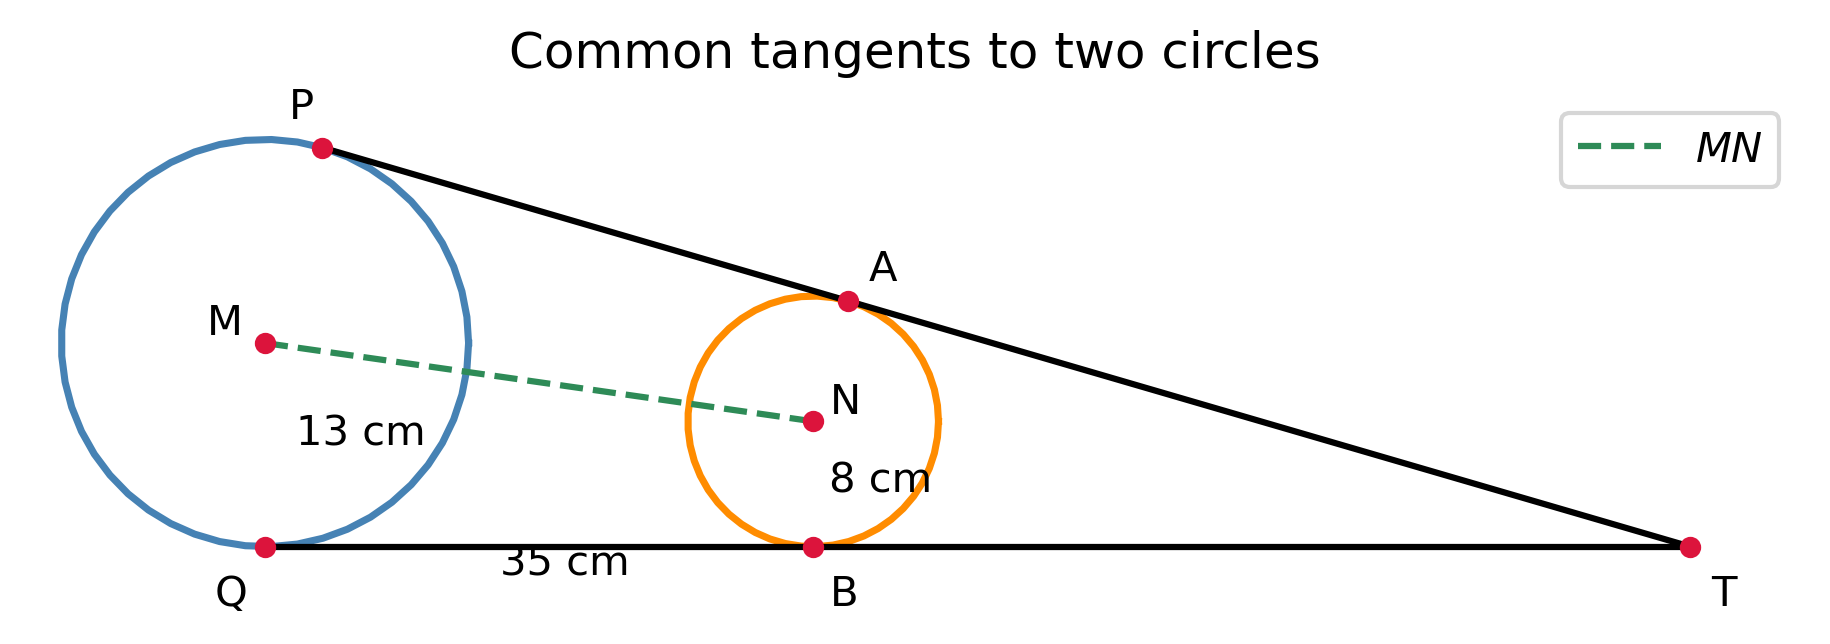
\includegraphics[width=0.38\linewidth]{figs/4.1.33.png}
    \caption{Schematic two-circle tangent configuration.}
\end{figure}
\end{enumerate}

\vspace{0.8em}
\begin{enumerate}[label={},font=\normalfont,leftmargin=1.15cm,labelwidth=1.0cm,labelsep=0.15cm,itemindent=0pt,listparindent=0pt,parsep=0pt,topsep=0pt]
\item[4.1.34] A kite is flying $60$ m above the ground. Ravi, on the roof of a house, holds the string straight and sees the kite at an angle of elevation of $30^\circ$. From the bottom of the building, the angle of elevation is $45^\circ$. Find the string length and the height of the roof. Use $\sqrt3=1.73$.

\vspace{0.7em}\par\solution


The $45^\circ$ angle from the building's bottom gives a horizontal distance of $60$ m to the kite's vertical projection. From the roof,
\begin{equation*}
\tan30^\circ=\frac{60-h}{60}\quad\Longrightarrow\quad h=60-20\sqrt3\approx25.4\text{ m}.
\tag*{(\ref{formula-1-1-11})}\end{equation*}
The string length is
\[
\sqrt{60^2+(20\sqrt3)^2}=40\sqrt3\approx69.2\text{ m}.
\]

The code draws the right-triangle configuration and calculates both lengths.
\begin{lstlisting}[frame=single, basicstyle=\rmfamily, escapeinside={(*@}{@*)}]
(*@\makebox[\dimexpr\linewidth-2\fboxsep-2\fboxrule\relax][c]{codes/4.1.34.py}@*)
\end{lstlisting}
\begin{figure}[H]
    \centering
    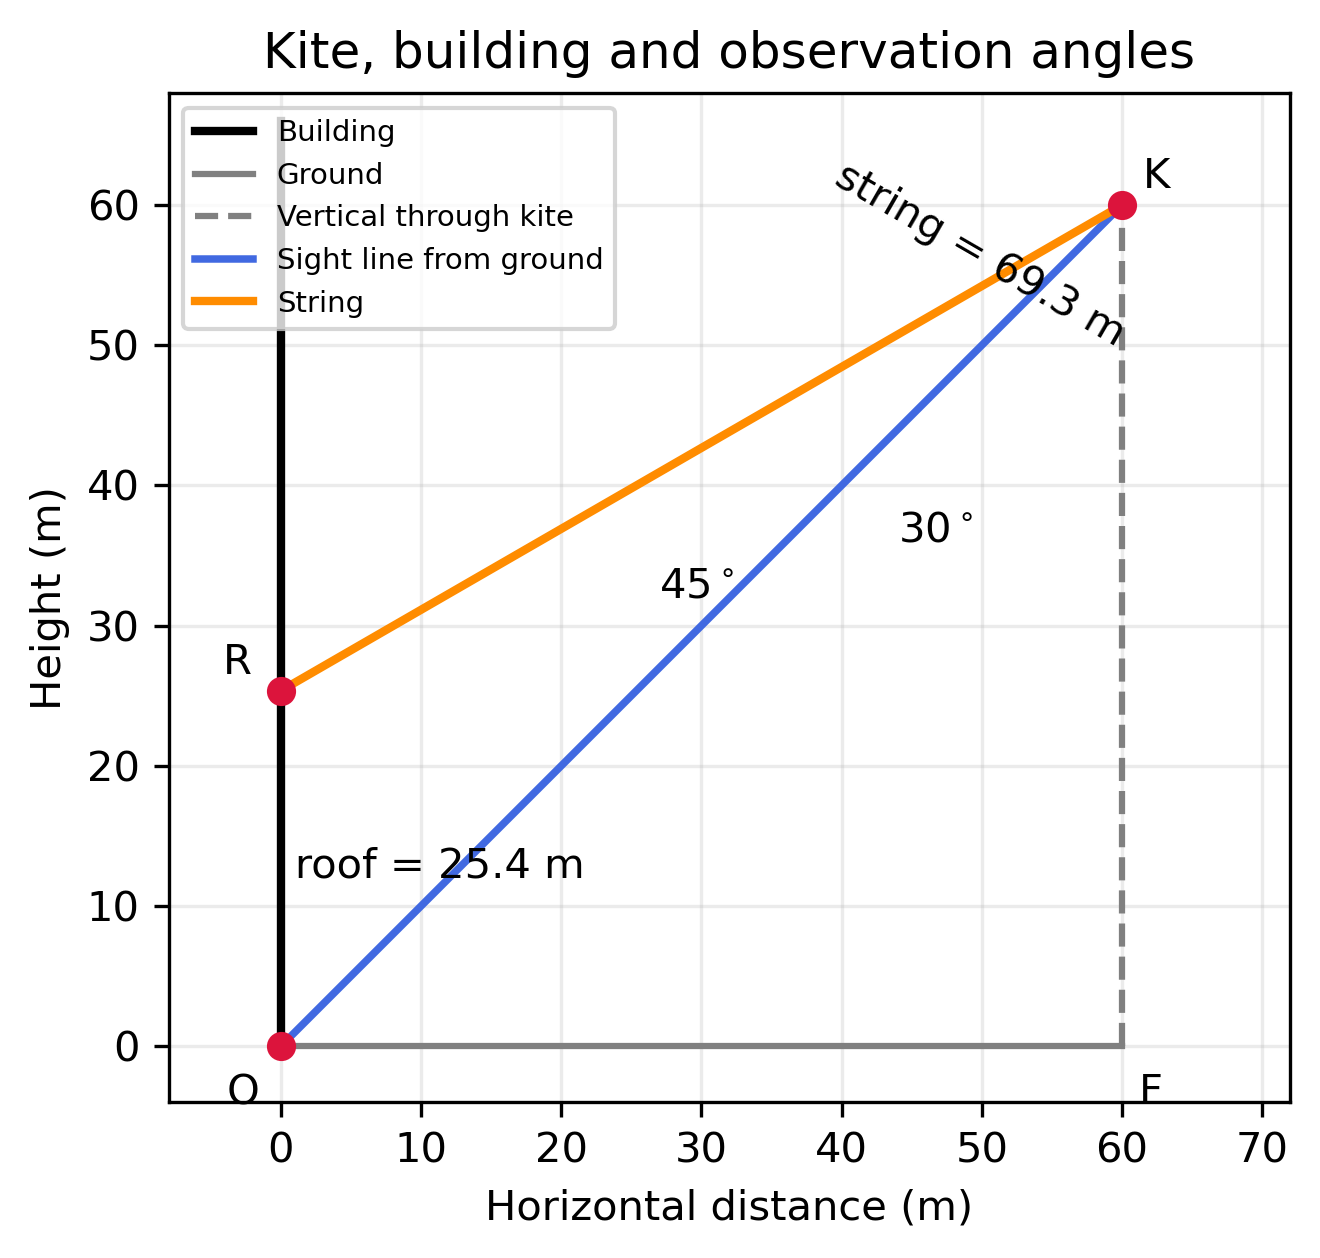
\includegraphics[width=0.40\linewidth]{figs/4.1.34.png}
    \caption{Kite and building geometry, with the two angles of elevation.}
\end{figure}
\end{enumerate}

\vspace{0.8em}
\begin{enumerate}[label={},font=\normalfont,leftmargin=1.15cm,labelwidth=1.0cm,labelsep=0.15cm,itemindent=0pt,listparindent=0pt,parsep=0pt,topsep=0pt]
\item[4.1.37] A Kolam pattern has successive dot counts $4,8,12,\ldots$. Find (i) the A.P.'s first term and common difference, (ii) its $n$th term, and (iii)(a) the number of squares formed with $220$ dots, or (b) whether $100$ dots can form a whole number of squares.

\vspace{0.7em}\par\solution


The counts form an A.P. with $a=4$, $d=4$, and $a_n=4n$. The total is $S_n=2n(n+1)$. For $220$ dots, $2n(n+1)=220$, so $n=10$. For $100$ dots, $n(n+1)=50$ has no integer solution; hence a whole number of squares cannot be completed.\par\noindent\hfill\mbox{\textit{(\ref{formula-1-1-8})}}\par

The C program calculates the A.P. terms and checks both totals.
\begin{lstlisting}[frame=single, basicstyle=\rmfamily, escapeinside={(*@}{@*)}]
(*@\makebox[\dimexpr\linewidth-2\fboxsep-2\fboxrule\relax][c]{codes/4.1.37.c}@*)
\end{lstlisting}
\end{enumerate}

\vspace{0.8em}
\begin{enumerate}[label={},font=\normalfont,leftmargin=1.15cm,labelwidth=1.0cm,labelsep=0.15cm,itemindent=0pt,listparindent=0pt,parsep=0pt,topsep=0pt]
\item[4.1.38] On a Cartesian map of Jaipur, Rambagh Palace is the origin. The locations are $A=(-4,2)$ (Rajasthan High Court), $B=(4,-4)$ (Birla Mandir), $C=(4,3)$ (Heera Bagh), and $D=(-5,-2)$ (Amar Jawan Jyoti). Find: (i) the daily distance from Heera Bagh to the court and back; (ii) the ratio in which the $x$-axis divides $AD$; (iii)(a) whether Birla Mandir is equidistant from Heera Bagh and Amar Jawan Jyoti, or (b) show using the section formula that $A,O,B$ are not collinear.

\vspace{0.7em}\par\solution


(i) $AC=\sqrt{(4+4)^2+(3-2)^2}=\sqrt{65}$, so the round trip is $2\sqrt{65}\approx16.12$ map units.\\
(ii) $A$ and $D$ have $y$-coordinates $2$ and $-2$, so the $x$-axis bisects $AD$ in the ratio $1:1$.\\
(iii)(a) $BC=7$, while $BD=\sqrt{9^2+2^2}=\sqrt{85}$. These are unequal, so Birla Mandir is not equidistant from $C$ and $D$.\\
Alternatively, for (iii)(b), the point dividing $AB$ in the ratio $1:1$ is, by the section formula, $\bigl(\frac{-4+4}{2},\frac{2-4}{2}\bigr)=(0,-1)$. Since $A$ and $B$ have opposite $x$-coordinates, any point on $AB$ with $x=0$ must divide it in ratio $1:1$. This point is not $O=(0,0)$, so $A,O,B$ are not collinear.\par\noindent\hfill\mbox{\textit{(\ref{formula-1-1-2}, \ref{formula-1-1-10})}}\par

The code plots the four locations, origin, and the segments used in the answers.
\begin{lstlisting}[frame=single, basicstyle=\rmfamily, escapeinside={(*@}{@*)}]
(*@\makebox[\dimexpr\linewidth-2\fboxsep-2\fboxrule\relax][c]{codes/4.1.38.py}@*)
\end{lstlisting}
\begin{figure}[H]
    \centering
    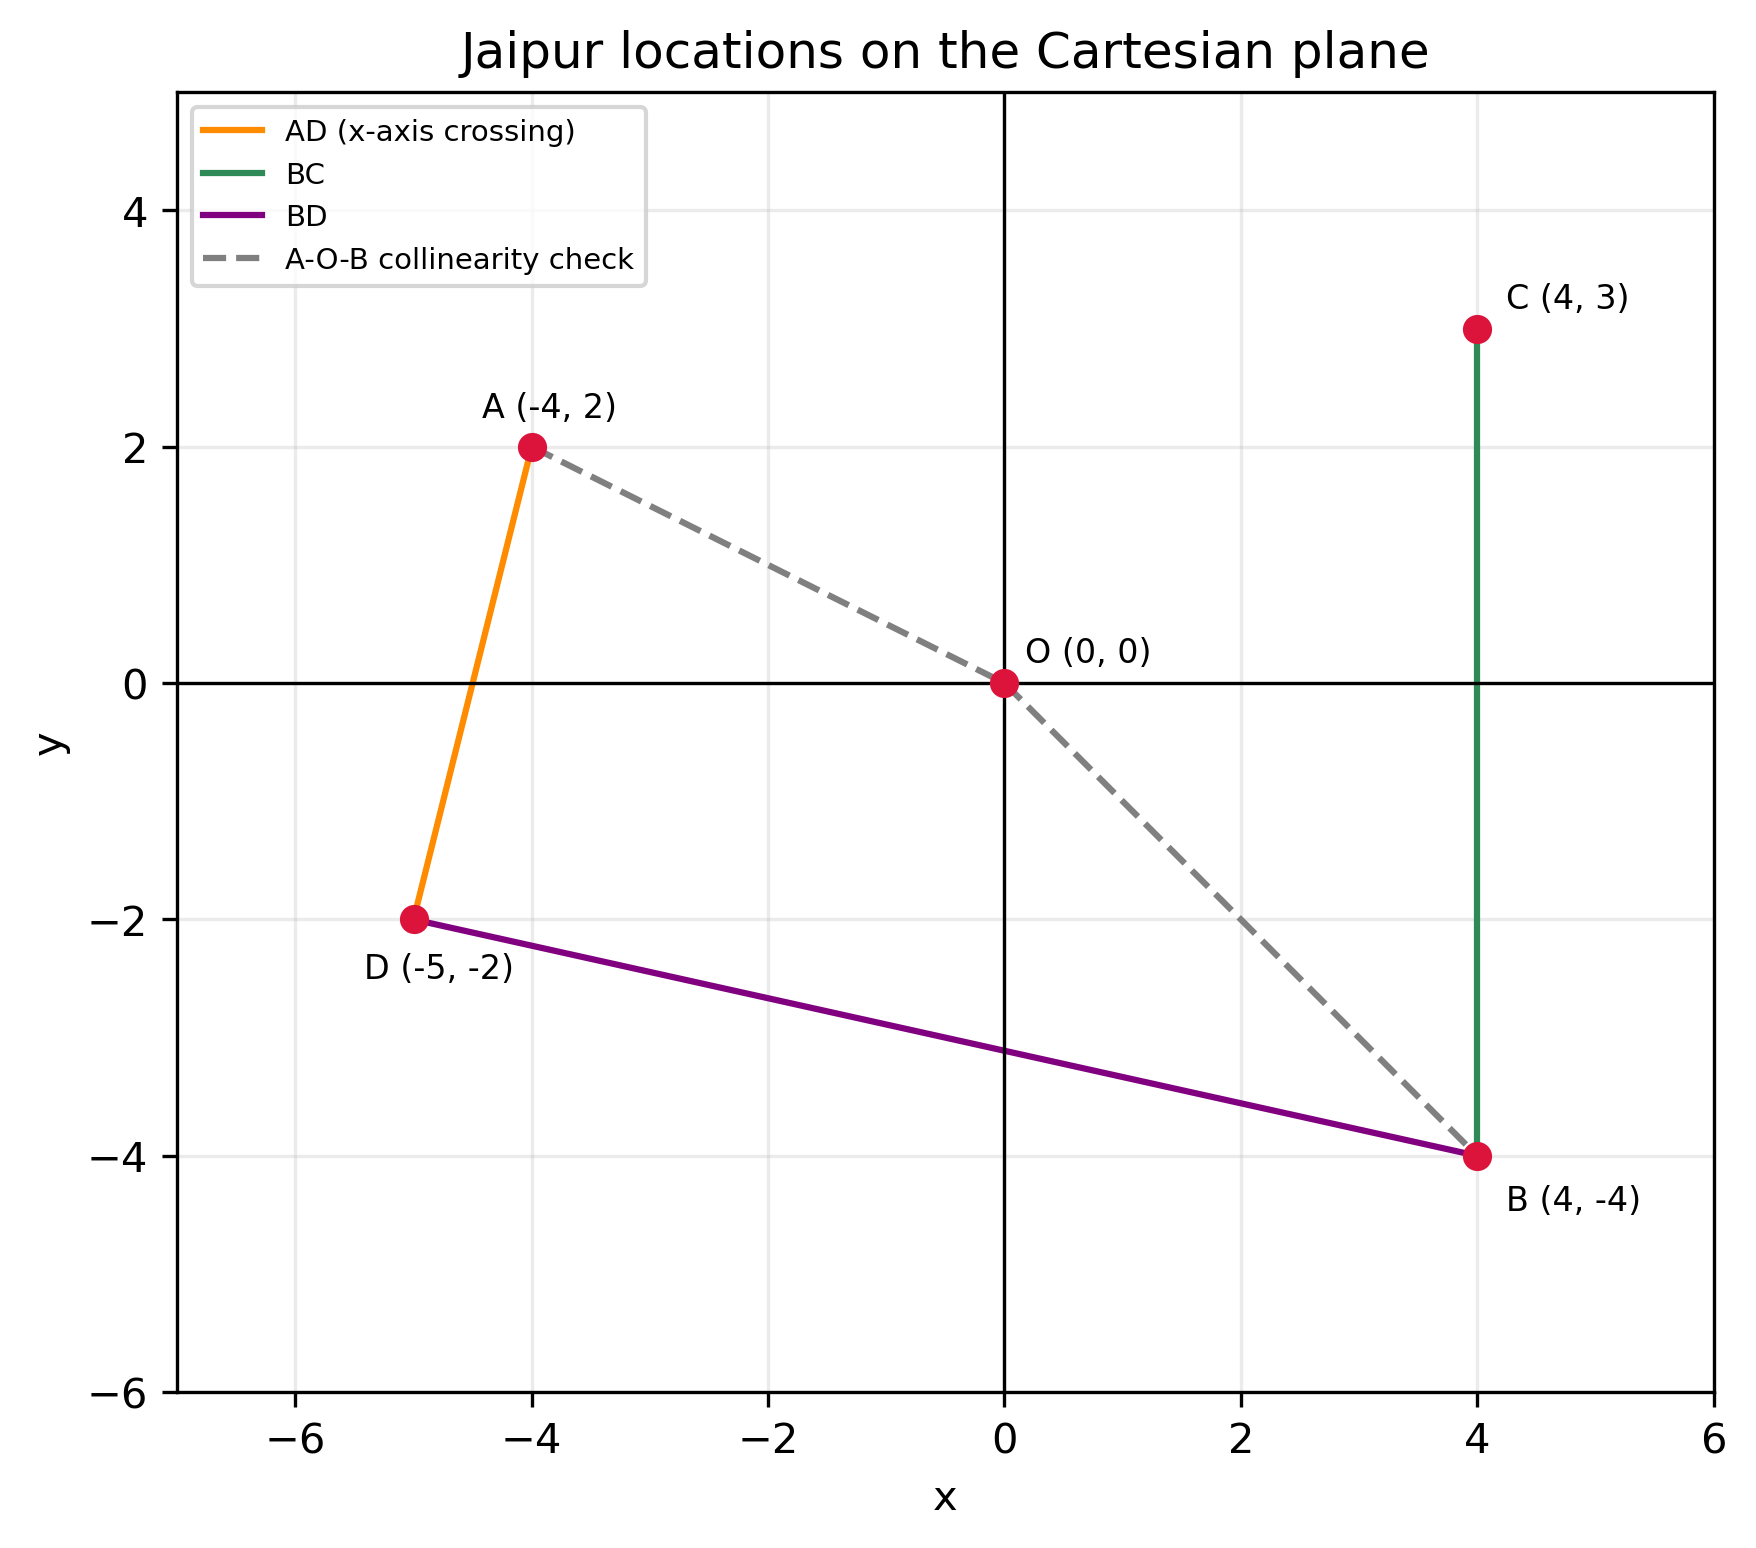
\includegraphics[width=0.48\linewidth]{figs/4.1.38.png}
    \caption{Jaipur locations plotted on the Cartesian plane.}
\end{figure}
\end{enumerate}